\chapter{Ergebnisse}
\section{Überblick}
Der genetische Algorithmus wurde mit einer Populationsgröße von 50 über 30 Generationen hinweg optimiert. Dabei konnte sowohl die Genauigkeit minimal verbessert werden als auch die Fehler reduziert. Der genetische Algorithmus konvergiert sehr schnell zum Ergebnis. Die Ausführung dauerte 14 Stunden. Dabei handelte es sich um die Konfiguration mit einer einer geringeren Standardabweichung bei der Rekombination, das bedeutet, dieser Lauf fokussierte sich mehr auf die Exploitation. Im Anhang finden sich die Resultate zum Lauf der Exploration.

\begin{figure}[h]
	\centering
	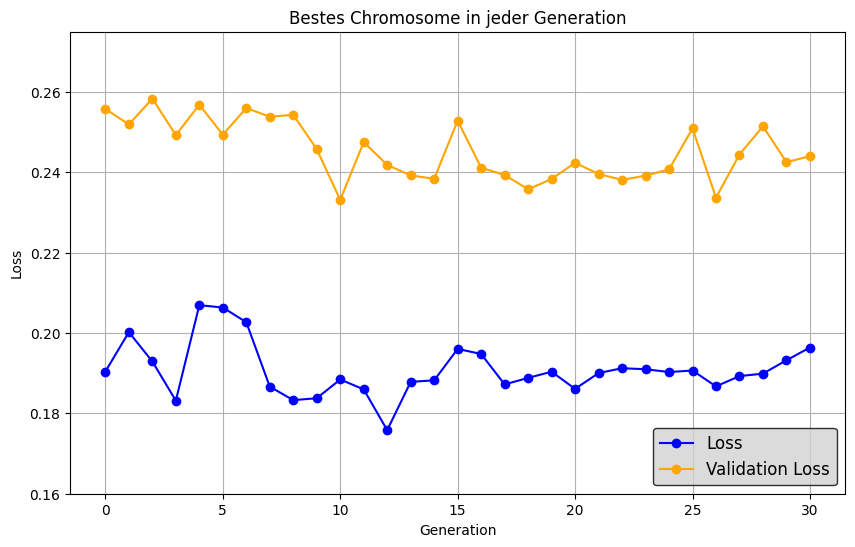
\includegraphics[width=1\linewidth]{loss.png}
	\caption{Geringster Fehler pro Generation}
	\label{fig:enter-label}
\end{figure}


\section{Interpretation der Ergebnisse}
Die Testergebnisse sind nicht wirklich aussagekräftig, denn die Fitness-Berechnung ist leider nicht deterministisch. So kann es passieren, dass ein Elitist, der gerade noch einen Fehler von 0.24 hatte, in der nächsten Generation einen Fehler von 0.23 ermittelt. Die Startkonfiguration der Neuronen sind zufällig und so fließt leider auch eine gewisse nicht-deterministische Komponente in die Fitness-Funktion ein. Dies wurde deutlicher, wenn probiert wurde, das beste Individuum zu reproduzieren: hierbei wurde oft ein schlechterer Wert erreicht. Das gute Ergebnis kam daher durch einen optimaleren Bias im Neuron.

Insgesamt konnte das Netz nicht merklich verbessert werden, dies könnte an der geringen Auswahl der Hyperparameter liegen. Wahrscheinlich wäre es besser ein tieferes Netz mit mehr Schichten zu nehmen, in welcher dann auch die Neuronenanzahl optimiert werden, dies würde aber auch den Suchraum extrem erweitern. Karlupia et. al. hatten Erfolge bei der Benutzung eines genetischen Algorithmus zur Optimierung eines CNN für die Gesichtserkennung. CNN's haben durch die Faltungs- und Pooling-Schichten deutlich mehr Hyperparameter zum Optimieren. \parencite{karlupia_genetic_2023}. 

Das rein zufällige Erstellen der Generationen nach "Random Grid Search", führt daher zu einen ähnlichen Ergebnis. Es liegt also nahe, dass die Optimierung der vier Hyperparameter schlicht weg zu wenig war. Die Devianz der einzelne Läufe waren dafür zu hoch.

\section{Verbesserungsmöglichkeiten}
Eine Erhöhung der Gene im Chromosom führt zu einem erweiterten Suchraum und mehr Dimensionen, so würde der Unterschied zu Grid Search, welches öfters Probleme mit einer hohen Anzahl von Dimensionen hat, größer werden. Daher erscheint es sinnvoll mehr Hyperparameter aufzunehmen. 

\section{Vergleich zu Grid Search}
Um einen Vergleich zu einer anderen Hyperparameter-Optimierungen bekommen wurde das gleiche neuronale Netz mittels Grid Search optimiert. Hierfür wurden die einzelnen Parameter im gleichen Intervall rasterförmig verstreut und ausprobiert. Dabei wurden um die 700 Kombinationen der Parameter ausgeführt und deren Genauigkeit/Fehler verglichen. Dabei wurde beobachtet, dass diese Brute Force Herangehensweise bei einem solch kleinen Netz zu ähnlich guter Konfiguration führt. 

\section{Fazit}
Genetische Algorithmen erweisen gute Dienste bei dem Optimierungsproblem, allerdings sollte drauf geachtet werden den Suchraum nicht zu klein zu lassen. Wenn es die Problemstellung zulässt, dann sollte am besten der Suchraum erst ausreichend groß skaliert werden. Wenn dann in gegebener Zeit keine gute Lösung gefunden wird, dann kann der Suchraum auch verkleinert werden. 
